\documentclass[11pt, a4paper]{article}
\usepackage{pdfpages}
\usepackage{parallel}
\usepackage[T2A]{fontenc}
%\usepackage{ucs}
\usepackage[utf8]{inputenc}
\usepackage[english,russian]{babel}
\usepackage{hyperref}
\usepackage{rotating}
\usepackage[inner=2cm,top=1.8cm,outer=2cm,bottom=2.3cm,nohead]{geometry}
%\usepackage{listings}
\usepackage{graphicx}
\usepackage{wrapfig}
\usepackage{longtable}
\usepackage{indentfirst}
\usepackage{array}
\usepackage{tikzsymbols}
\usepackage{soul}
\usepackage[ruled,vlined]{algorithm2e}
\usepackage{qrcode}
\counterwithout{figure}{section} 

\usepackage{url}
\makeatletter
\g@addto@macro{\UrlBreaks}{\UrlOrds}
\makeatother

\newcolumntype{P}[1]{>{\raggedright\arraybackslash}p{#1}}
\frenchspacing
%\usepackage{fixltx2e} %text sub- and superscripts
\usepackage{icomma} % коскі ў матэматычным рэжыме
%\PreloadUnicodePage{4}

\newcommand{\longpage}{\enlargethispage{\baselineskip}}
\newcommand{\shortpage}{\enlargethispage{-\baselineskip}}

\def\switchlang#1{\expandafter\csname switchlang#1\endcsname}
\def\switchlangbe{
\let\saverefname=\refname%
\def\refname{Літаратура}%
\def\figurename{Іл.}%
}
\def\switchlangru{
\let\saverefname=\refname%
\let\savefigurename=\figurename%
\def\refname{Литература}%
\def\figurename{Рис.}%
}
\def\switchlangen{
\let\saverefname=\refname%
\def\refname{References}%
\def\figurename{Fig.}%
}

\hyphenation{admi-ni-stra-tive}
\hyphenation{ex-pe-ri-ence}
\hyphenation{fle-xi-bi-li-ty}
\hyphenation{Py-thon}
\hyphenation{ma-the-ma-ti-cal}
\hyphenation{re-ported}
\hyphenation{imp-le-menta-tions}
\hyphenation{pro-vides}
\hyphenation{en-gi-neering}
\hyphenation{com-pa-ti-bi-li-ty}
\hyphenation{im-pos-sible}
\hyphenation{desk-top}
\hyphenation{elec-tro-nic}
\hyphenation{com-pa-ny}
\hyphenation{de-ve-lop-ment}
\hyphenation{de-ve-loping}
\hyphenation{de-ve-lop}
\hyphenation{da-ta-ba-se}
\hyphenation{plat-forms}
\hyphenation{or-ga-ni-za-tion}
\hyphenation{pro-gramming}
\hyphenation{in-stru-ments}
\hyphenation{Li-nux}
\hyphenation{sour-ce}
\hyphenation{en-vi-ron-ment}
\hyphenation{Te-le-pathy}
\hyphenation{Li-nux-ov-ka}
\hyphenation{Open-BSD}
\hyphenation{Free-BSD}
\hyphenation{men-ti-on-ed}
\hyphenation{app-li-ca-tion}

\def\progref!#1!{\texttt{#1}}
\renewcommand{\arraystretch}{2} %Іначай формулы ў матрыцы зліпаюцца з лініямі
\usepackage{array}

\def\interview #1 (#2), #3, #4, #5\par{

\section[#1, #3, #4]{#1 -- #3, #4}
\def\qname{LVEE}
\def\aname{#1}
\def\q ##1\par{{\noindent \bf \qname: ##1 }\par}
\def\a{{\noindent \bf \aname: } \def\qname{L}\def\aname{#2}}
}

\def\interview* #1 (#2), #3, #4, #5\par{

\section*{#1\\{\small\rm #3, #4. #5}}
\ifx\ParallelWhichBox\undefined%
    \addcontentsline{toc}{section}{#1, #3, #4}%
\else%
\ifnum\ParallelWhichBox=0%
    \addcontentsline{toc}{section}{#1, #3, #4}%
\fi\fi%

\def\qname{LVEE}
\def\aname{#1}
\def\q ##1\par{{\noindent \bf \qname: ##1 }\par}
\def\a{{\noindent \bf \aname: } \def\qname{L}\def\aname{#2}}
}

\newcommand{\interviewfooter}[1]{
\vskip 1em
\noindent \textit{#1}
}

\AtEndDocument{\vfill\centering \qrcode{https://github.com/fiowro/mouses/blob/main/\jobname.pdf}}

\switchlang{en}
\begin{document}

\title{1986 "--- Honeywell/Asher quadLYNX trackball}
\date{}
\maketitle
\selectlanguage{english}
The quadLYNX trackball shown in fig. \ref{fig:quadLYNXPic} is a modification of the LX200 trackball designed for Apple Macintosh computers. The LX200, better known by its microLYNX and comLYNX variants, was released in California by Honeywell, a subsidiary of Disc Instruments; it proved to be a long-lived product, with many subsequent reissues under different brands, with different connection interfaces and electronics \cite{lx200}. Judging by the advertising materials, the quadLYNX model under the Honeywell brand appeared in 1986 \cite{honeywell}. However, in 1988, an advertisement in similar design appeared for this model as the ``LX200-192-D1'' under the Asher Engineering Corporation brand (mentioning Honeywell as the original developer of the device) \cite{asher}. To add to the confusion, in the same year Asher Engineering Corporation advertised a Turbo Trackball device -- exclusively under its own brand, in a differently shaped case, but with a strong similarity in the model number (``LX200-192-S3A'') and some of the internal design solutions \cite{turbo}.

\begin{figure}[h]
    \centering
    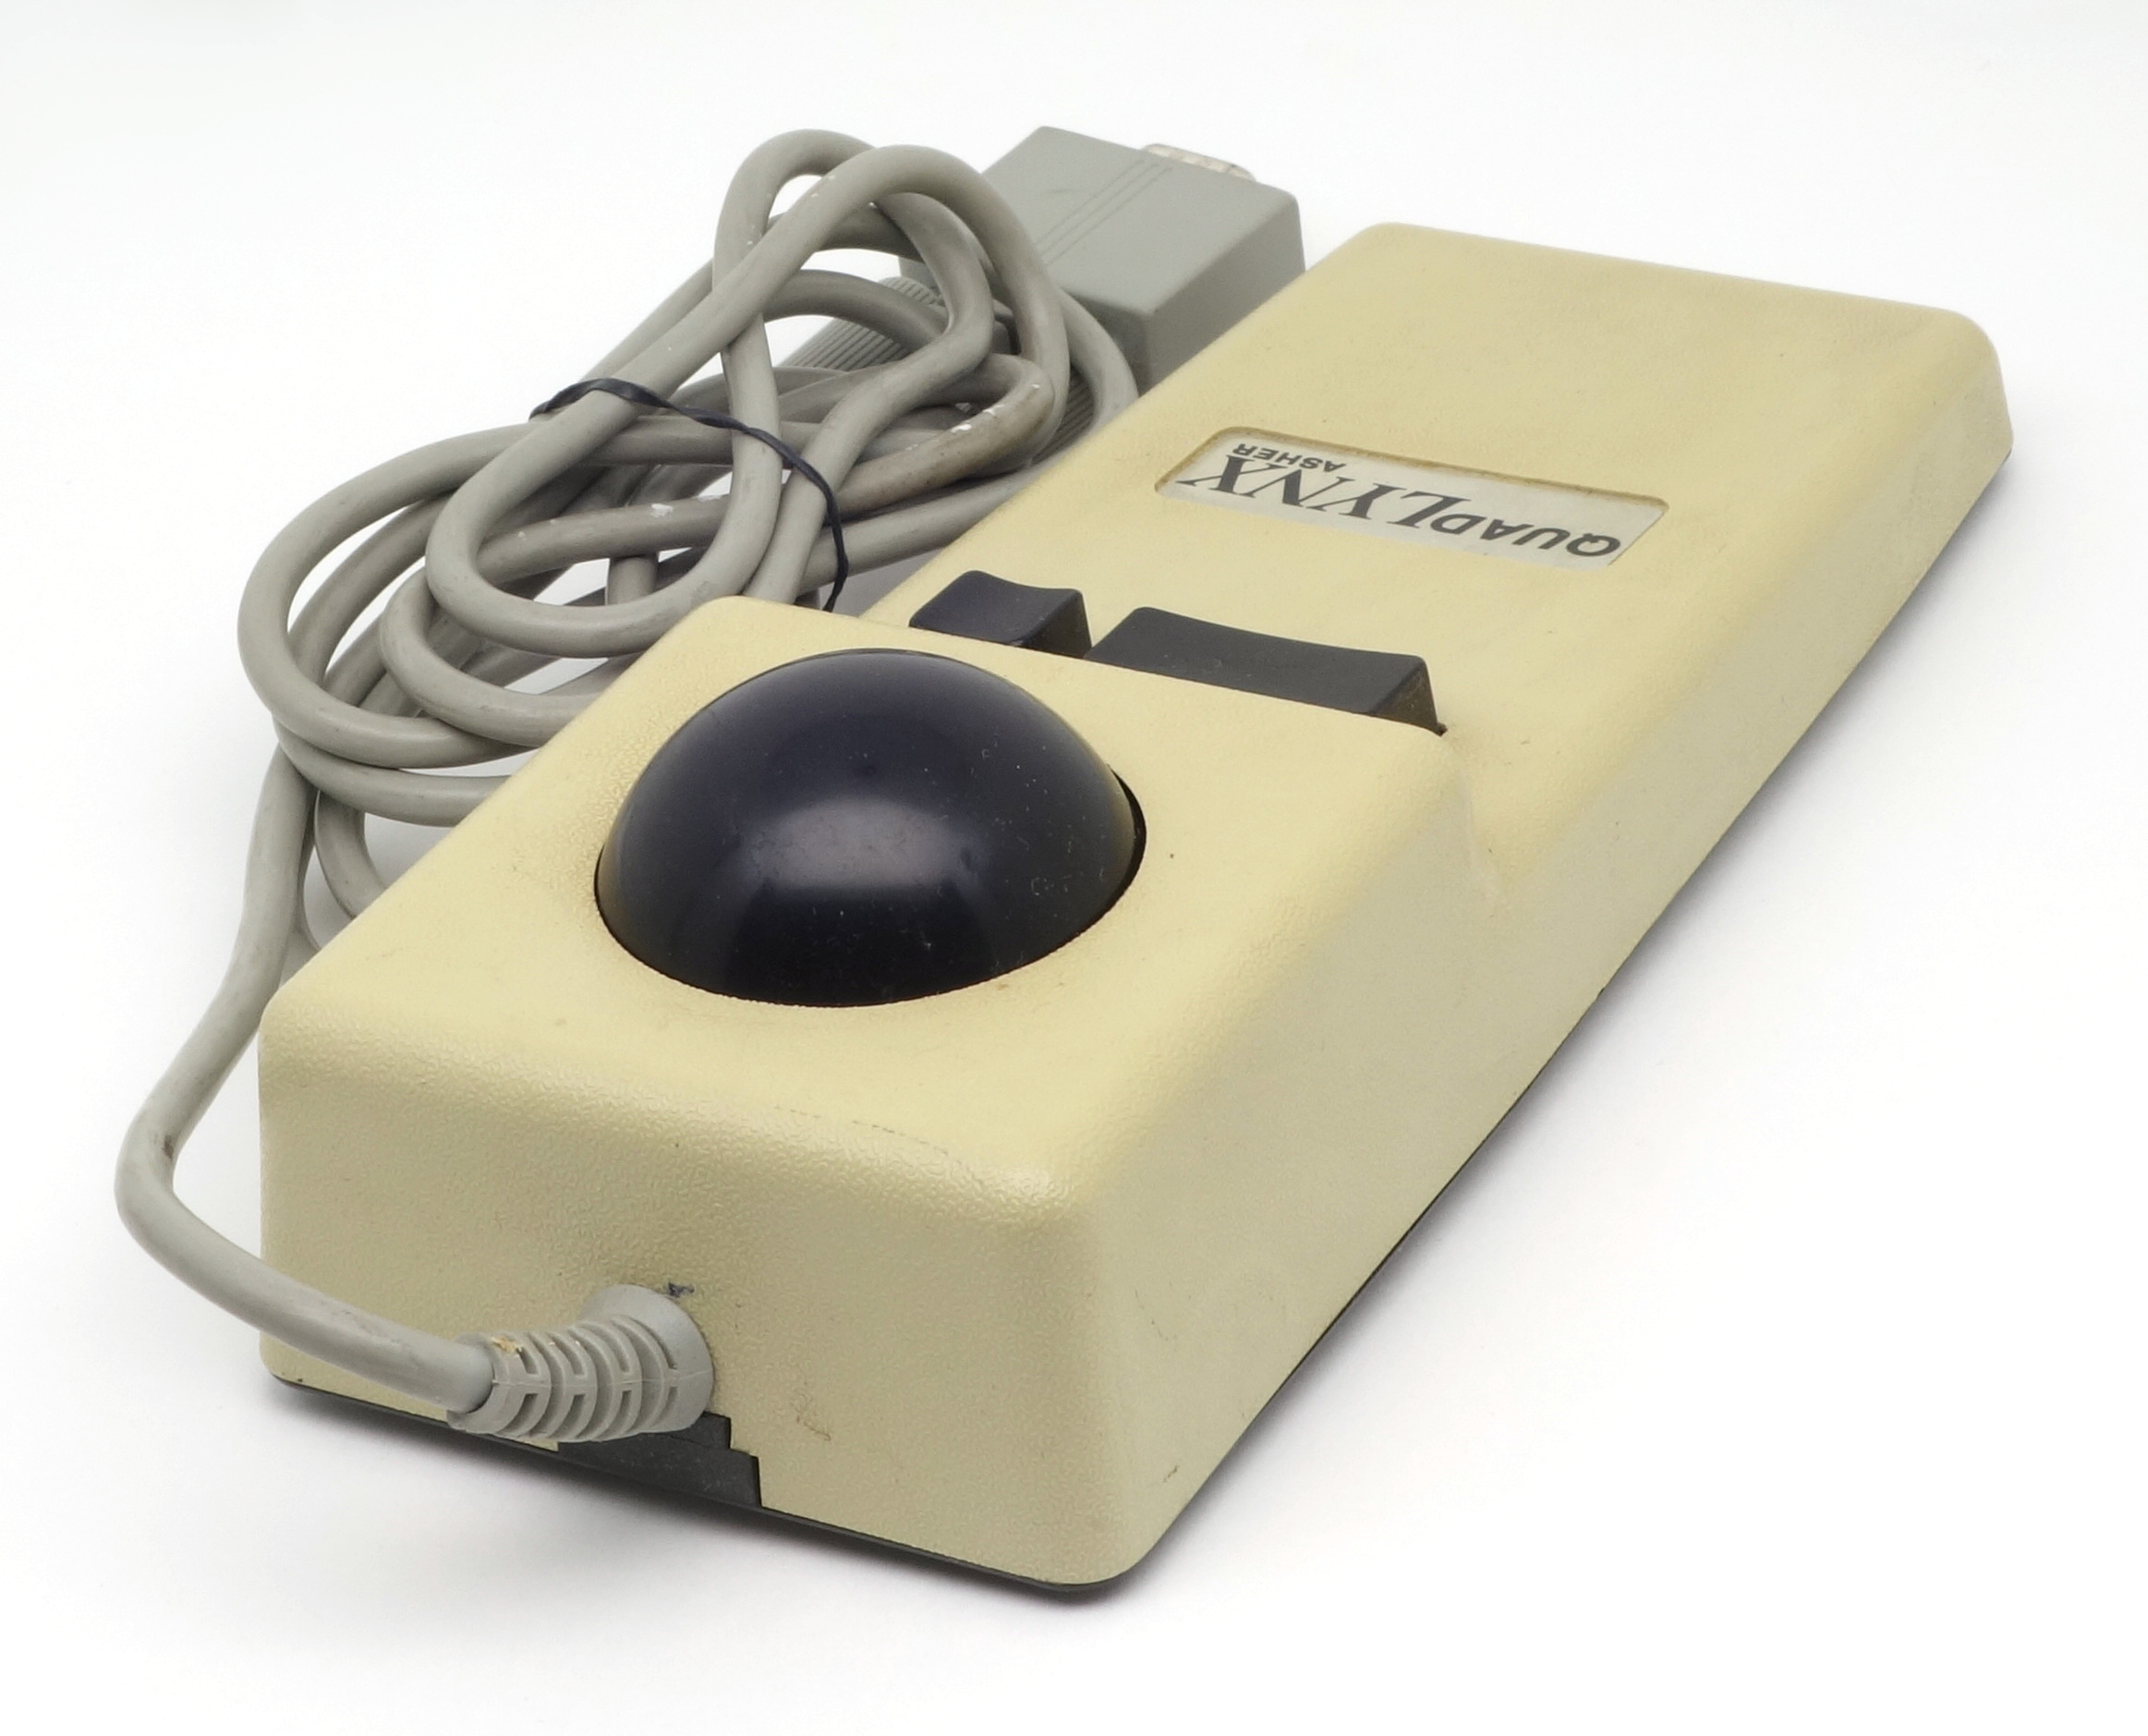
\includegraphics[scale=0.78]{1986_honeywell_asher_quadlynx_trackball/pic_30.jpg}
    \caption{Asher quadLYNX trackball}
    \label{fig:quadLYNXPic}
\end{figure}

The trackball has the typical LX200 design with a large black ball recessed into a beige body with an elongated wrist rest \ref{fig:quadLYNXTopBottom}. The ball fits snugly to the edges of the hole in the device case, which protects well from debris getting inside the trackball, but makes it impossible to remove the ball for cleaning without disassembling the case. In front of the ball are two buttons with keycaps identical to the keys of the classic full-size keyboard. This is the main visual difference between the quadLYNX and other LX200 variants equipped with three buttons.

\begin{figure}[h]
    \centering
    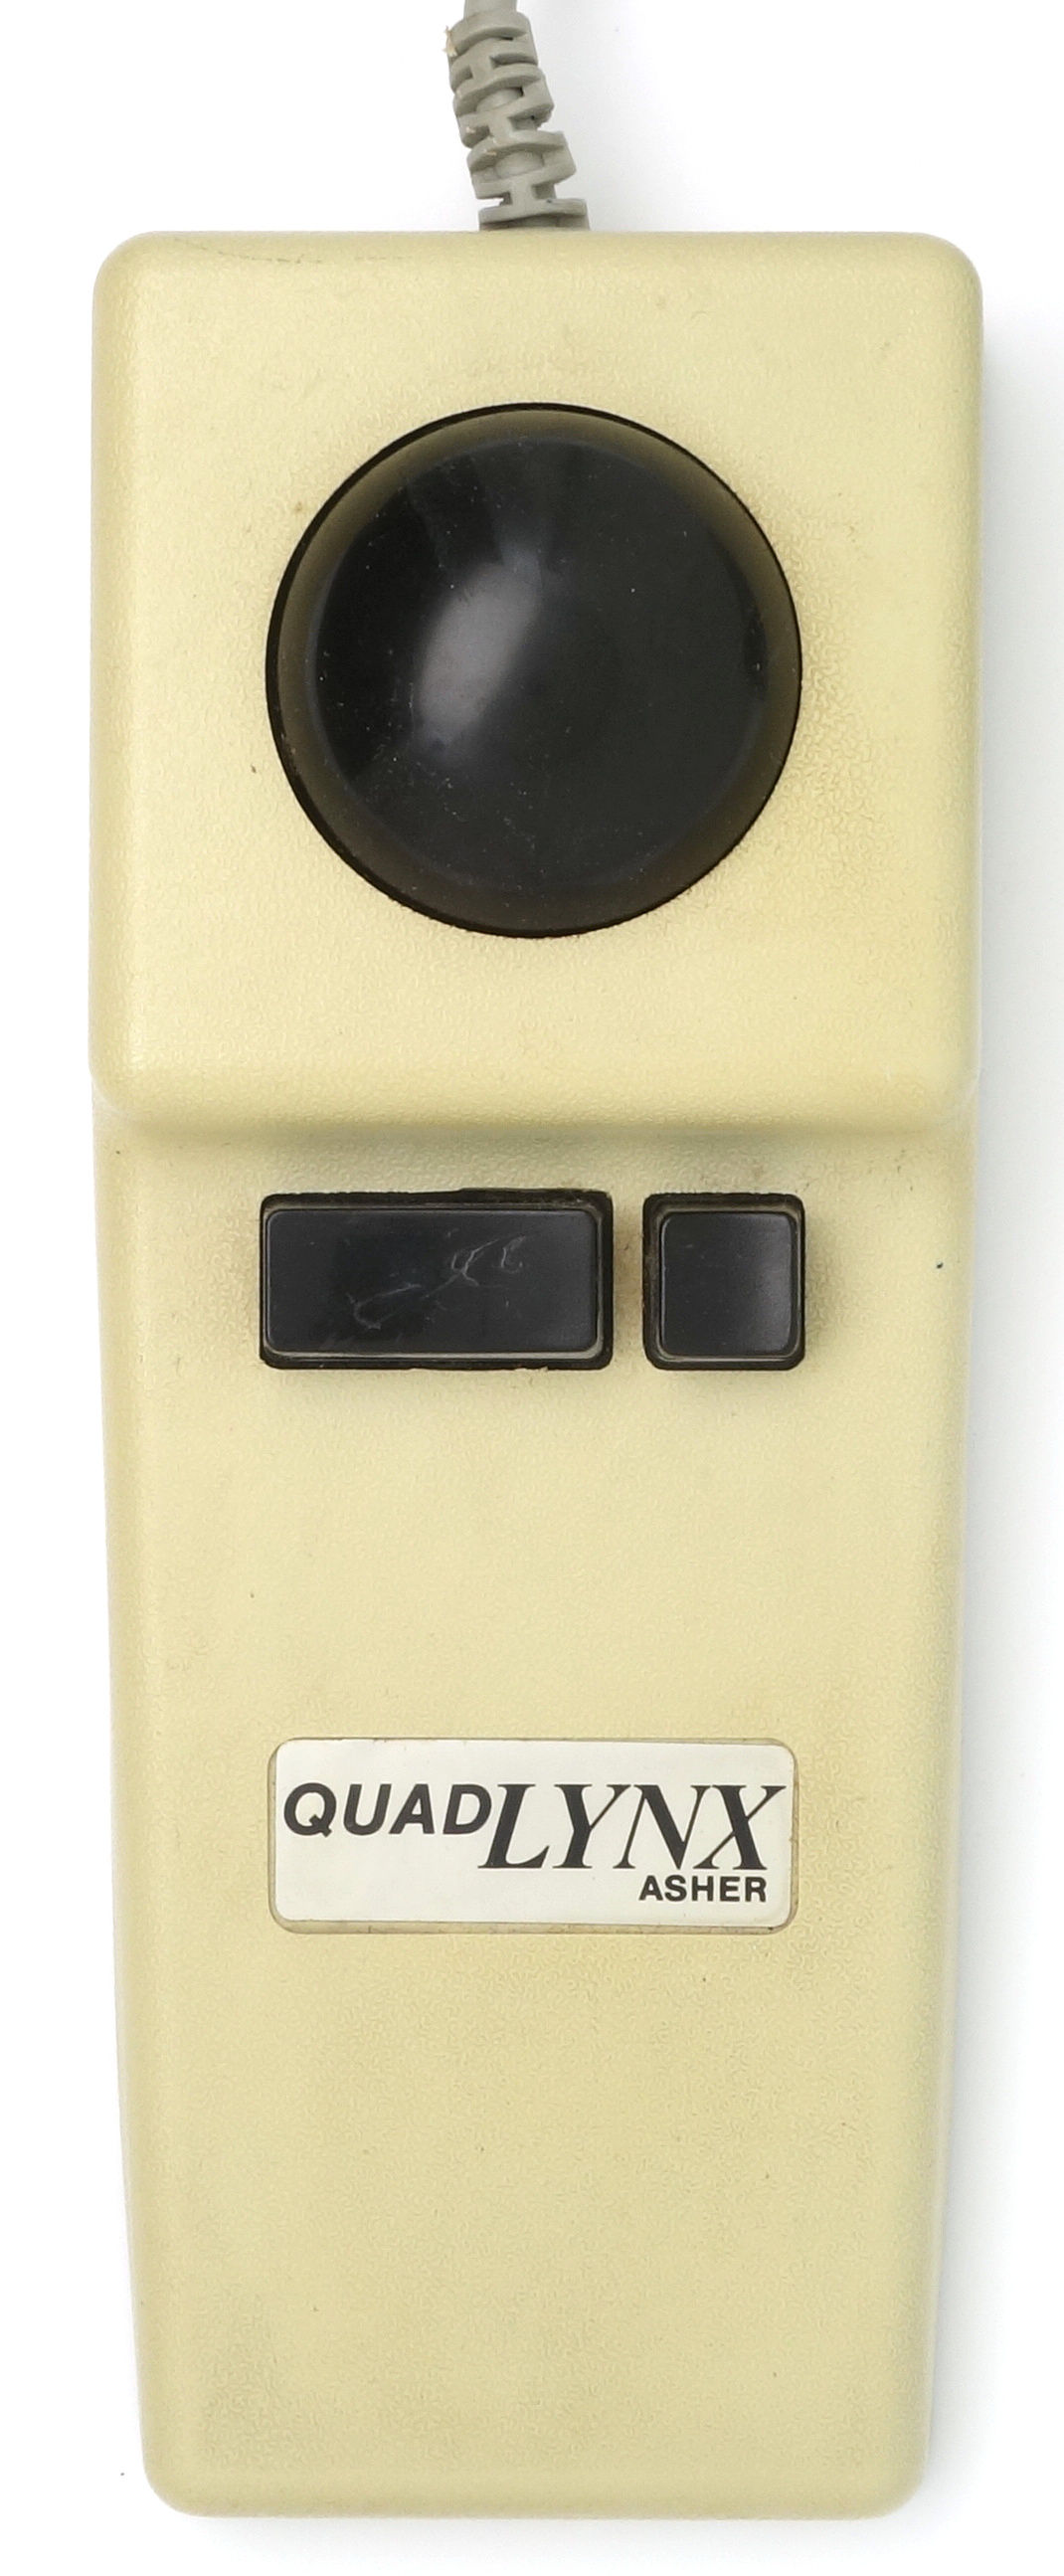
\includegraphics[scale=0.45]{1986_honeywell_asher_quadlynx_trackball/top_30.jpg}
    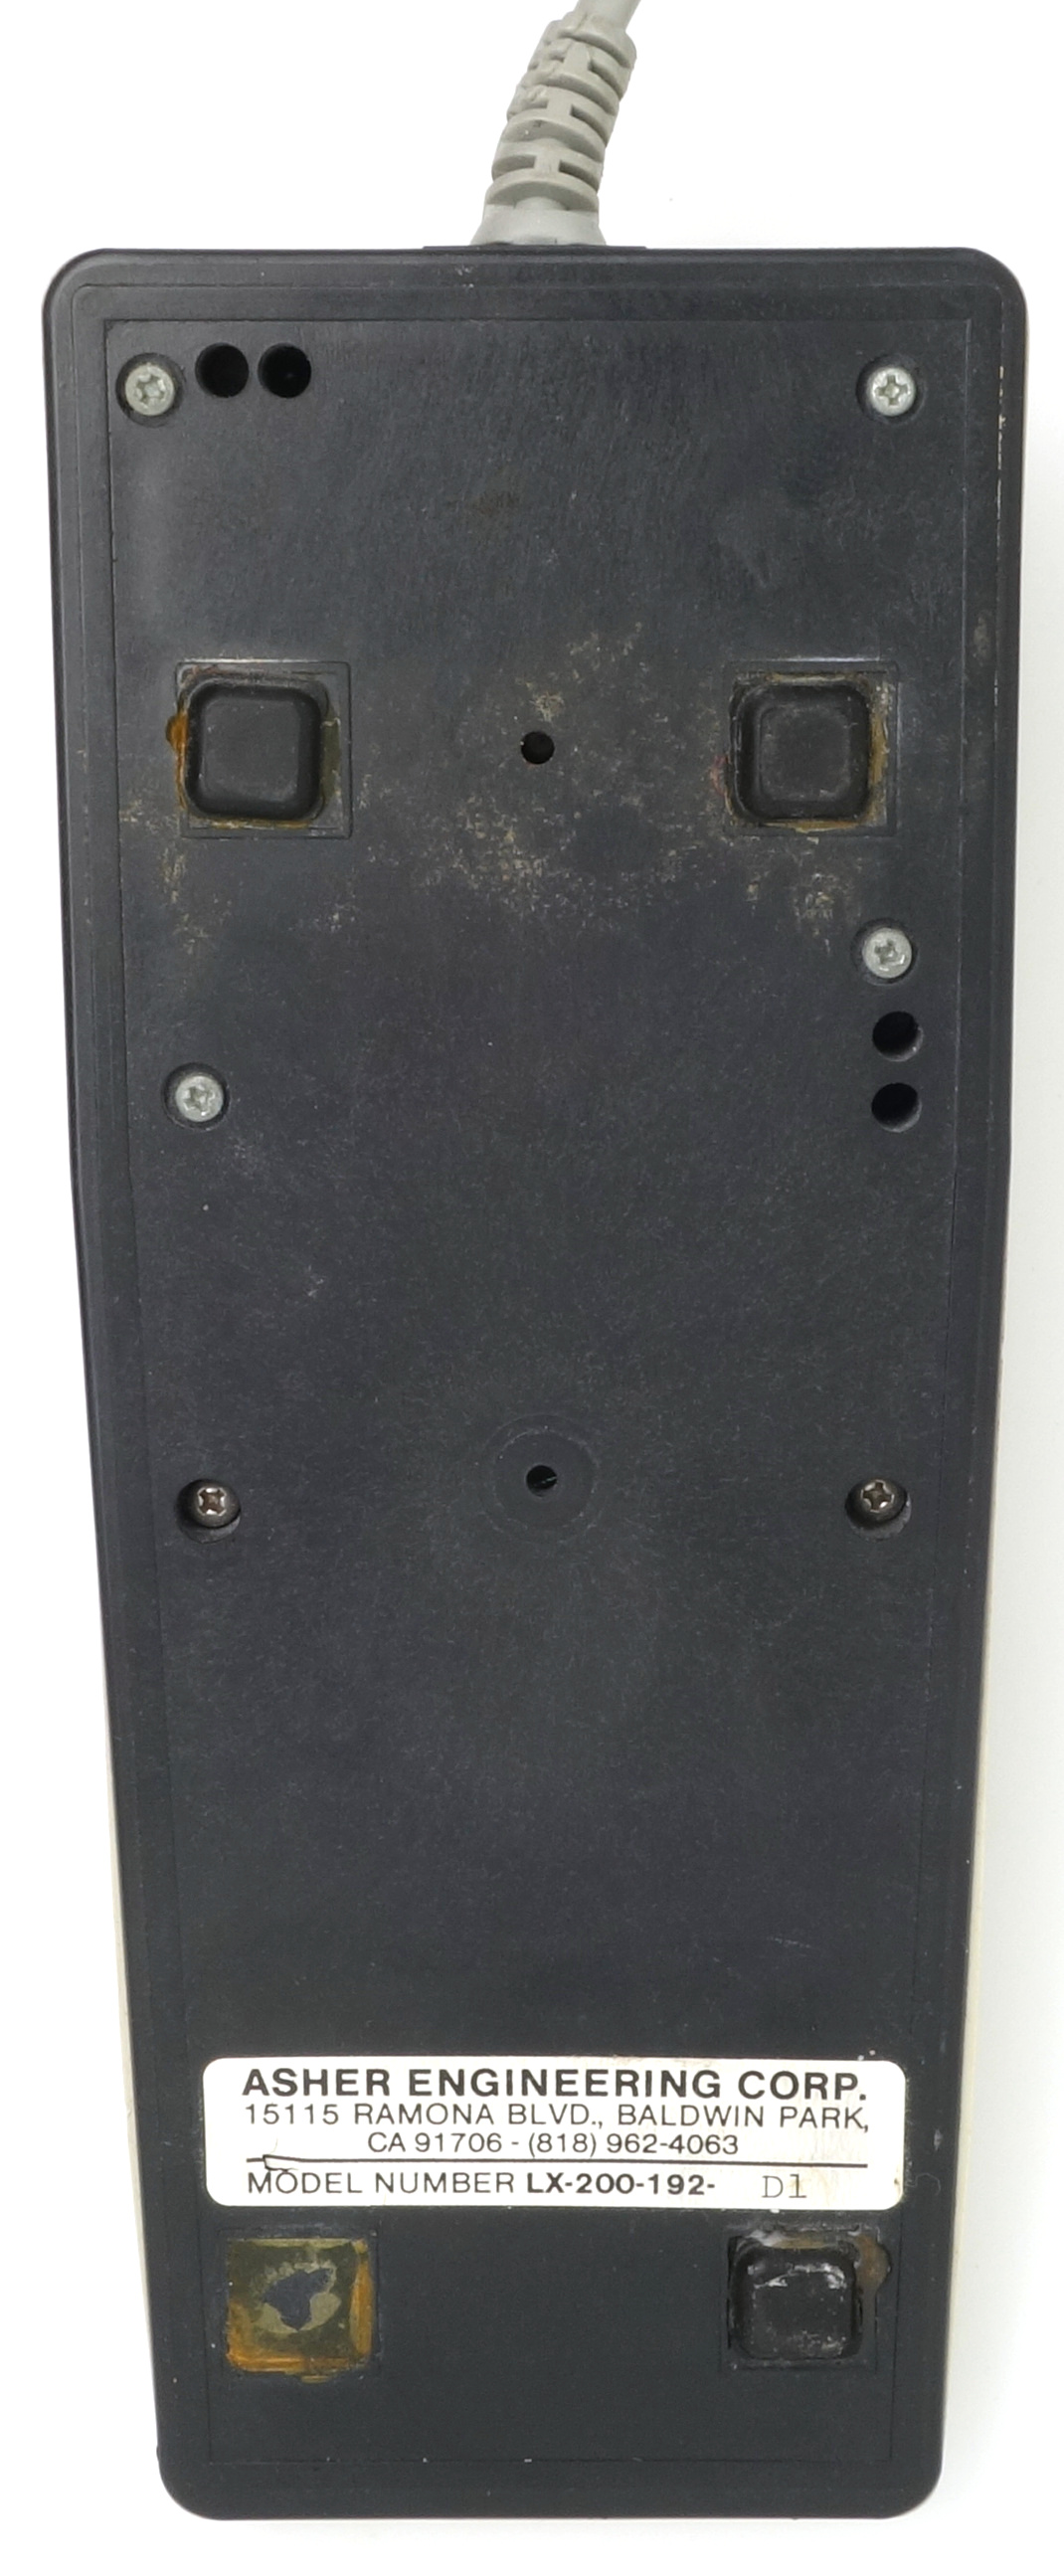
\includegraphics[scale=0.45]{1986_honeywell_asher_quadlynx_trackball/bottom_30.jpg}
    \caption{quadLYNX, top and bottom views}
    \label{fig:quadLYNXTopBottom}
\end{figure}

In terms of ergonomics, the dimensions of the trackball (fig. \ref{fig:quadLYNXSize}), as well as the rounded edges and corners, could create fairly comfortable working conditions.

\begin{figure}[h]
    \centering
    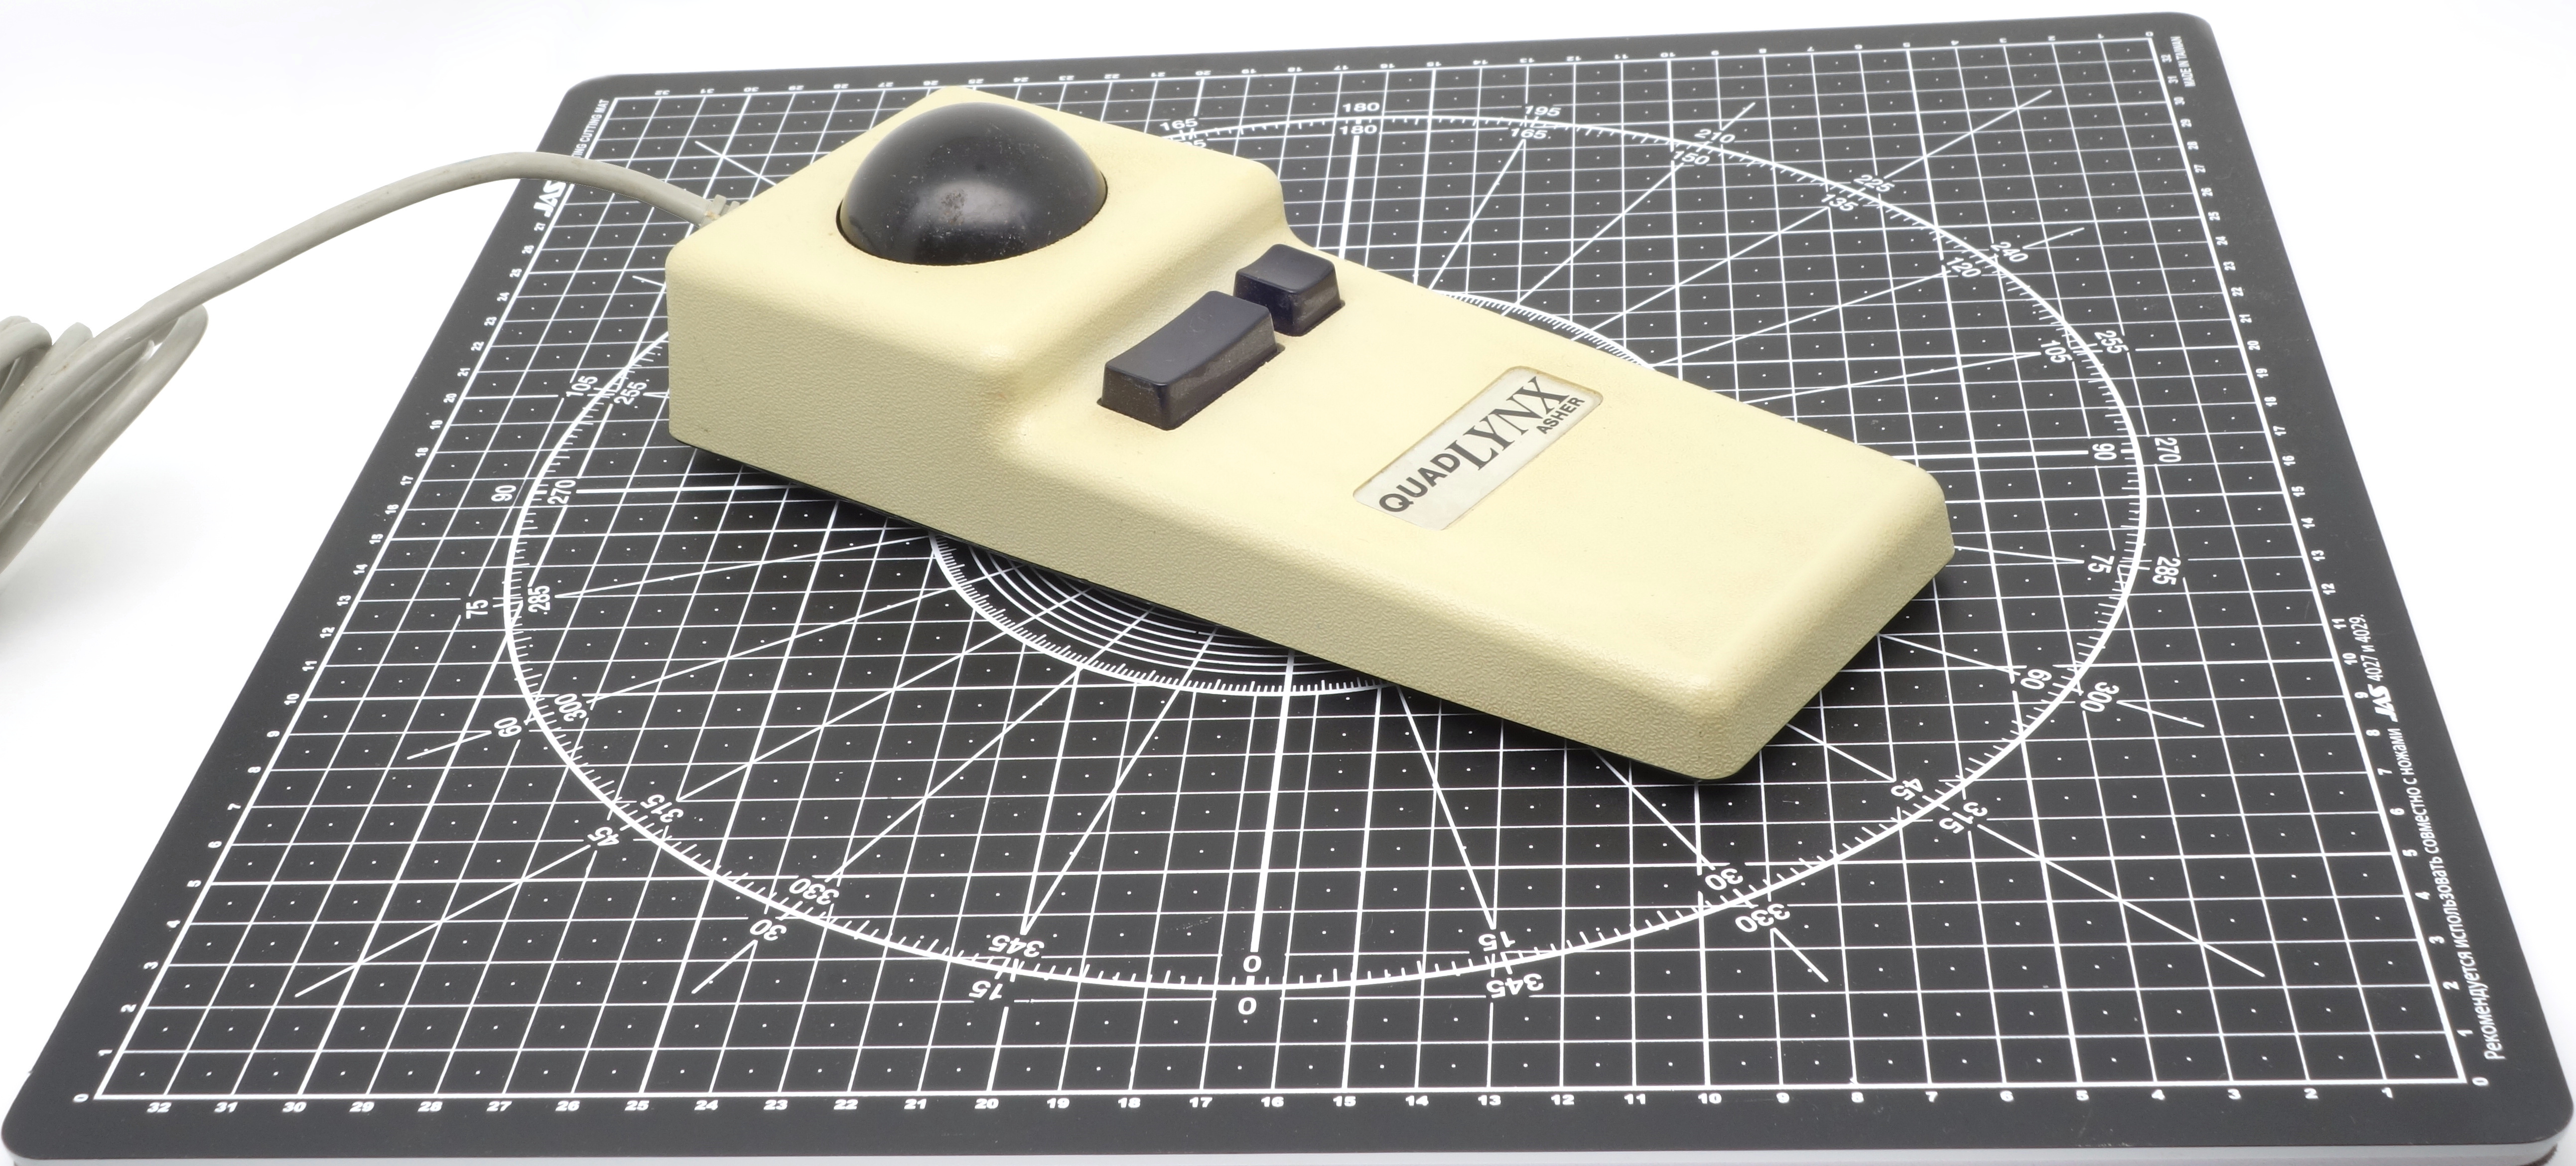
\includegraphics[scale=0.4]{1986_honeywell_asher_quadlynx_trackball/size_30.jpg}
    \caption{quadLYNX on a graduated pad with a grid step of 1~cm}
    \label{fig:quadLYNXSize}
\end{figure}

However, the buttons are far from the ball and their location is significantly lower, which deprives the user of the ability to press them with one hand without moving the wrist, or with both hands, since they are covered by the palm when the ball rotates (Fig. \ref{fig:quadLYNXHand}). This especially complicates drag and drop , which was widely used in the Macintosh computer interface, and the trackball was designed specifically for these computers. To reduce the problem, the smaller right button acts as a drag ``latch''. Pressing the latch button virtually fixes the main trackball button in the pressed position, and pressing either button again turns off this mode \cite{bible}.

\begin{figure}[h]
    \centering
    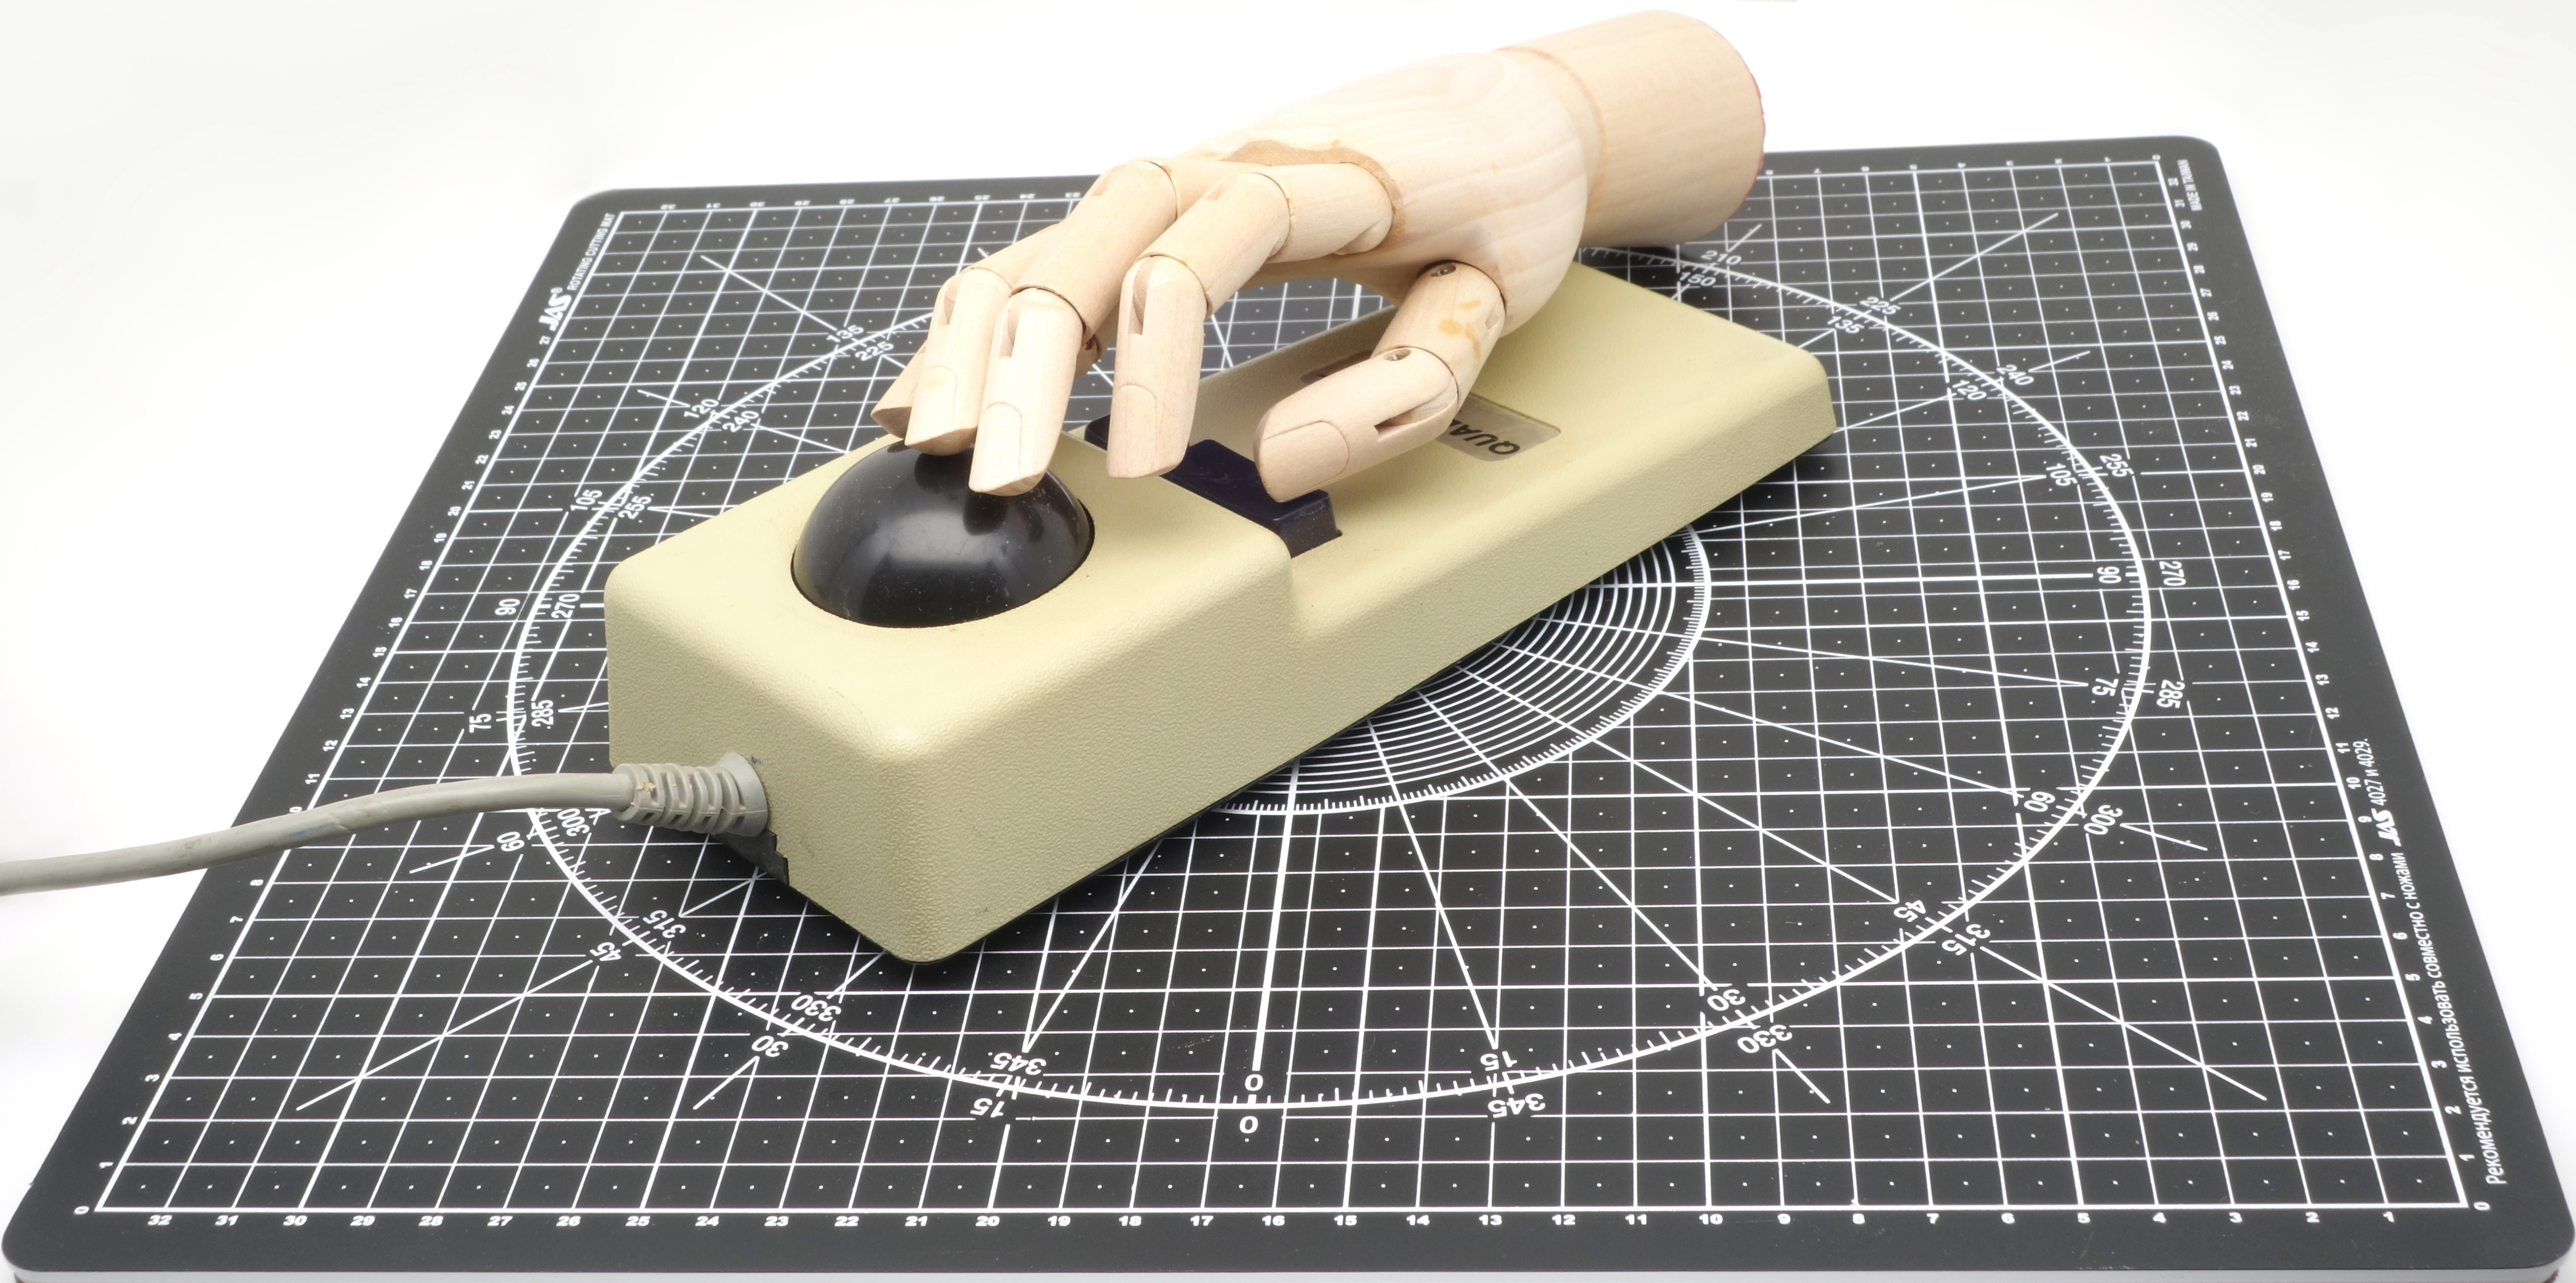
\includegraphics[scale=0.4]{1986_honeywell_asher_quadlynx_trackball/hand_30.jpg}
    \caption{quadLYNX with a human hand model}
    \label{fig:quadLYNXHand}
\end{figure}

Trackball internals are shown on figure \ref{fig:quadLYNXInside}. It is a mechanical encoder device, unlike most LX200 variants, which were equipped with an optomechanical encoder starting in the same year 1986. According to the information provided in \cite{lx200}, a mechanical encoder is sometimes found in early LX200s; in addition, the same ``patented hi-tech encoder used in sophisticated aerospace instrumentation'' \cite{turbo} can be found in the Asher Turbo Mouse trackball from 1988. 

As the image shows, the ``patented hi-tech encoder'' is a regular mechanical encoder disk covered with a plastic box on top, which makes it difficult for debris to get in (however, its design is not as hermetic and is noticeably less technologically advanced compared to, for example, closed mechanical encoders from ALPS Electric, used in early models of Microsoft, IBM and some other companies' mice).

\begin{figure}[h]
    \centering
    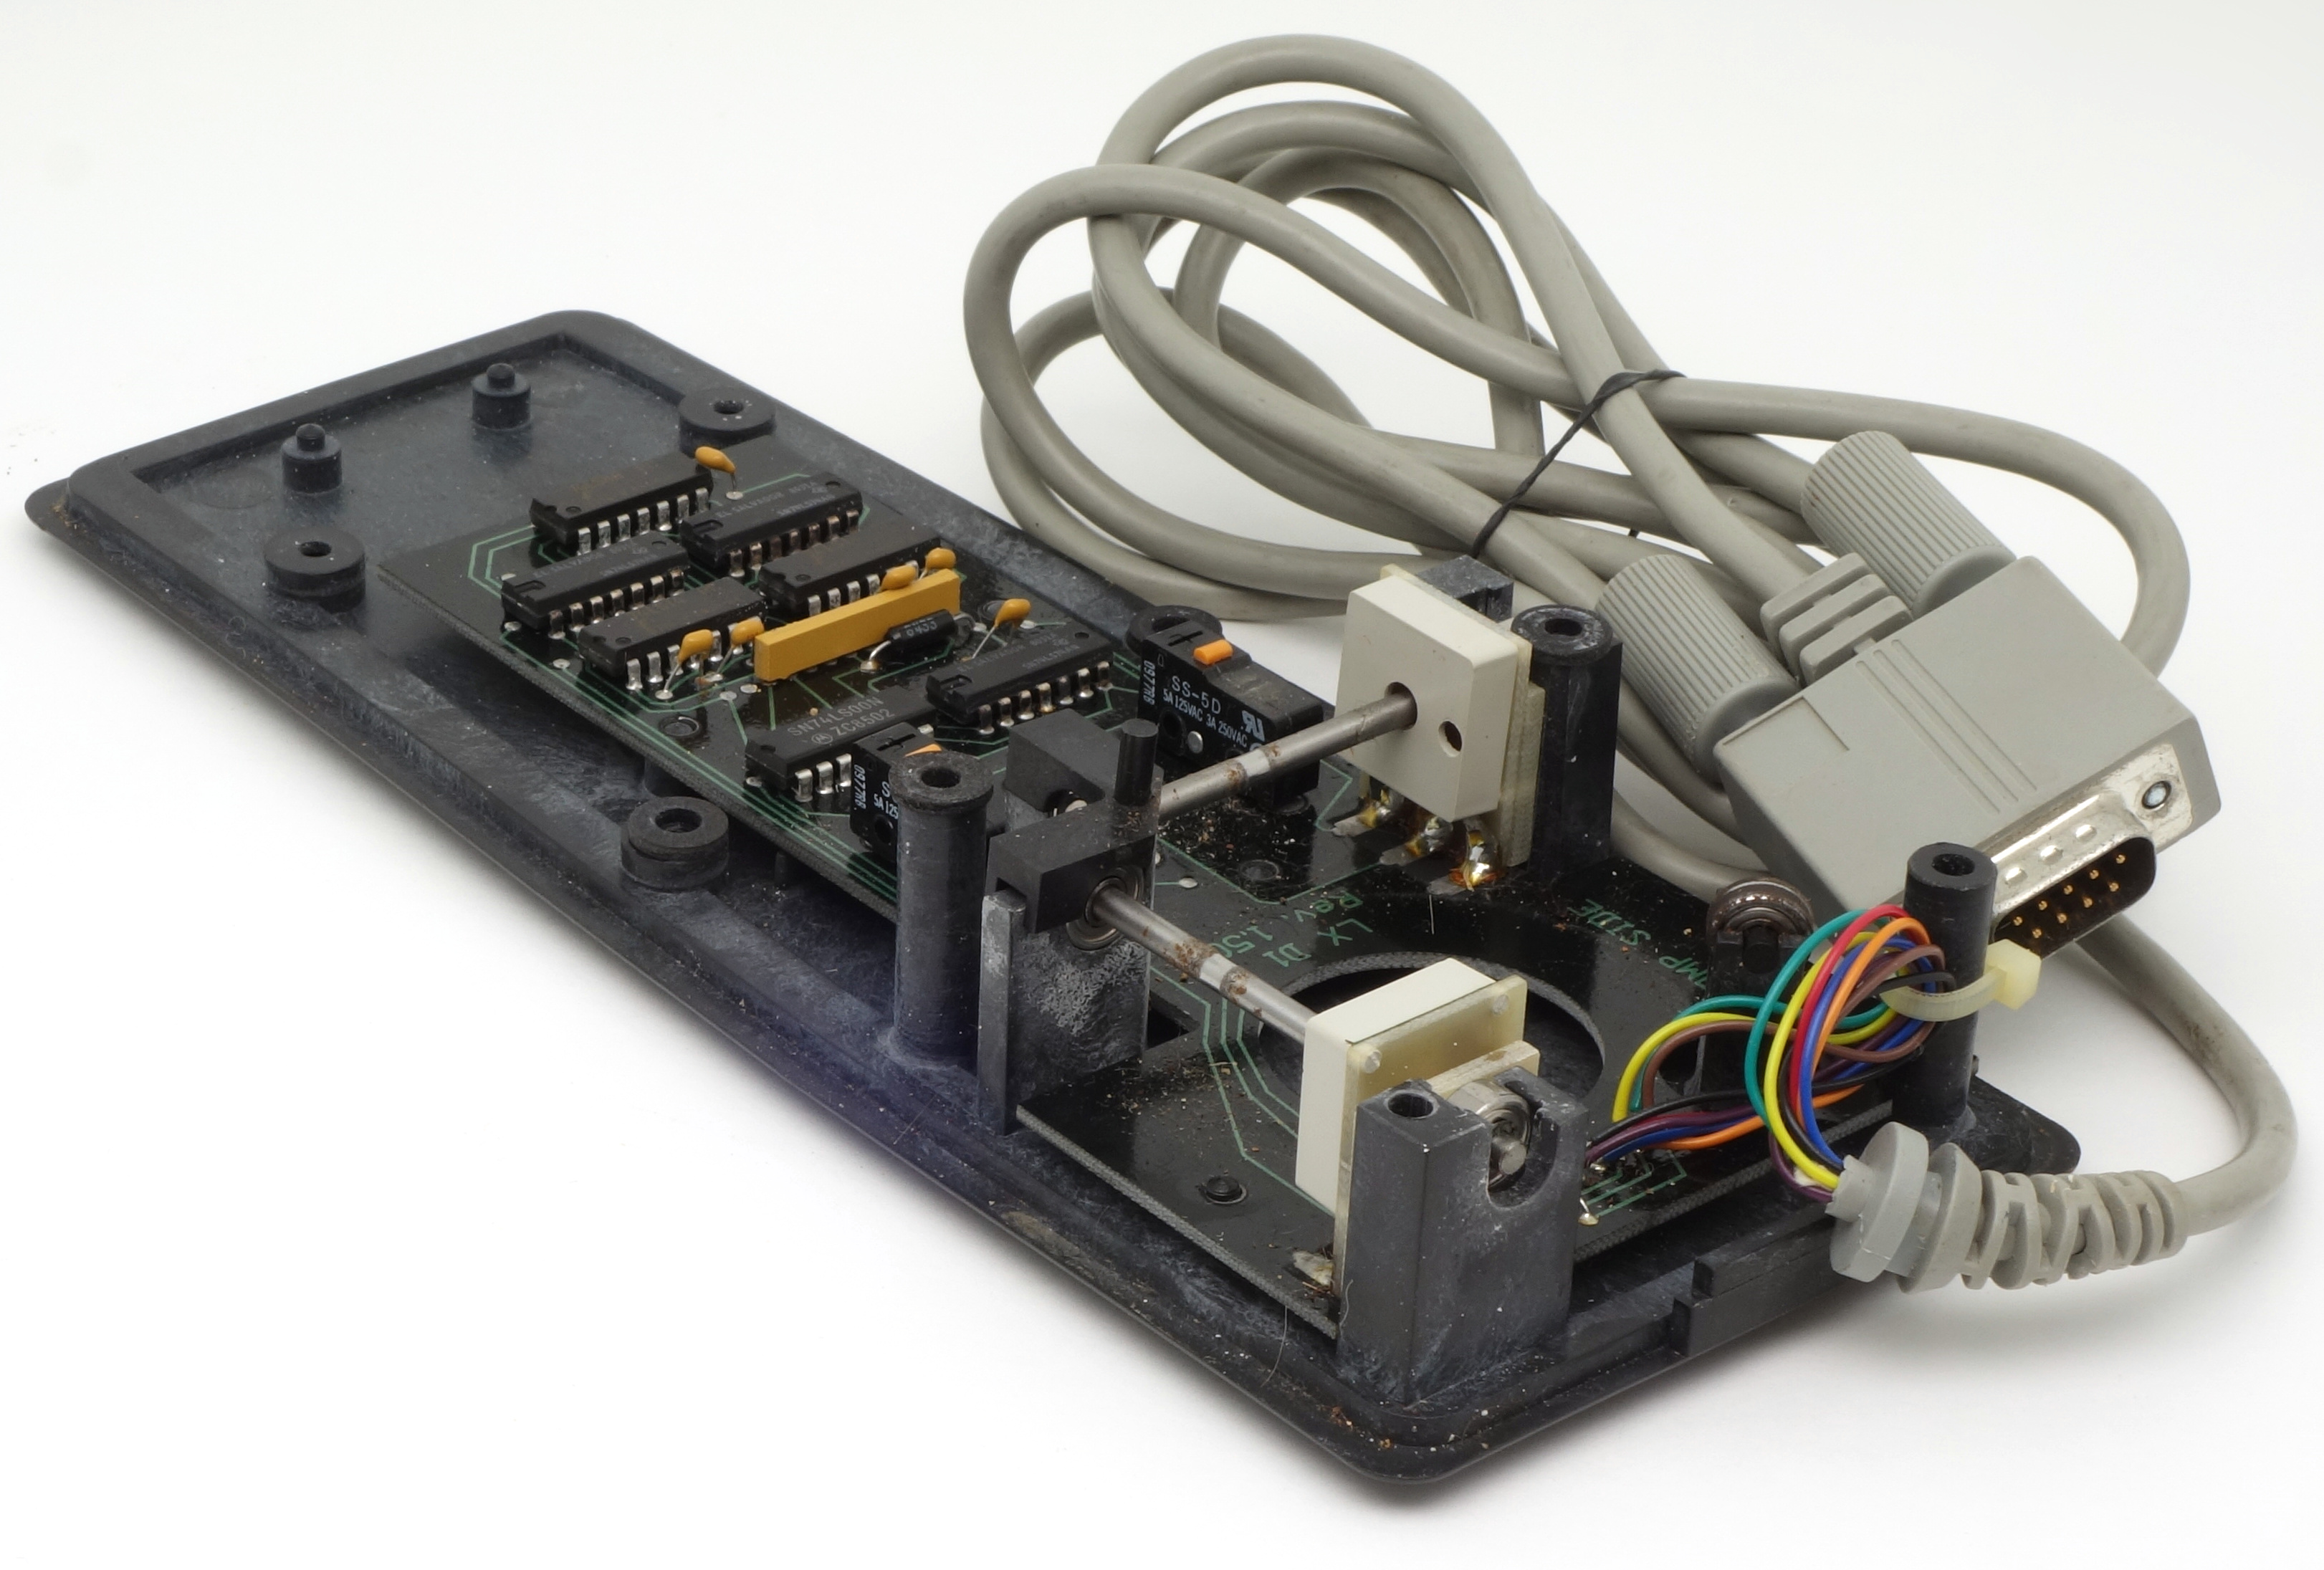
\includegraphics[scale=0.6]{1986_honeywell_asher_quadlynx_trackball/inside_30.jpg}
    \caption{quadLYNX disassembled}
    \label{fig:quadLYNXInside}
\end{figure}

Probably, the use of a mechanical encoder instead of optomechanics was aimed at reducing the cost of the device. However, the rest remained unchanged: the rollers are made using bearings and shafts made of stainless steel, ensuring high reliability and durability of the mechanical part of the device.

\begin{thebibliography}{9}
\bibitem {comlynx} Trackballs: Stationary mice // PC Magazine. August 1987, page 199-202 \url{https://trackballs.eu/media/Fulcrum/PC%20Mag%20Aug-1987%20p199-202.pdf}
\bibitem {lx200} Disc Instruments LX200 \url{https://web.archive.org/web/20220501213039/https://forum.trackballs.eu/viewtopic.php?f=17&t=16}
\bibitem {honeywell} Try the new quadLYNX Trackball // Macworld, August 1986. P. 155  \url{https://archive.org/details/eu_Macworld-1986-08_OCR/page/n155/mode/2up}
\bibitem {asher} Try the new quadLYNX Trackball // Macworld, January 1988. P. 212 \url{https://archive.org/details/macworld00unse_oel/page/212/mode/2up}
\bibitem {turbo} New Turbo Trackball from Asher // MacUser, February, 1988. P. 320 
\url{https://archive.org/details/MacUser8802February1988/page/n323/mode/2up}
\bibitem {bible} A. Naiman (ed.) QuadLYNX Trackball, Turbo Mouse. The Macintosh Bible. Chapter 2 -- Basic Mac hardware. PP. 73-75. \url{https://archive.org/details/macintoshbibleth00naim/page/72/mode/2up}
\end{thebibliography}
\end{document}
